\documentclass{standalone}
\usepackage{tikz}

\begin{document}
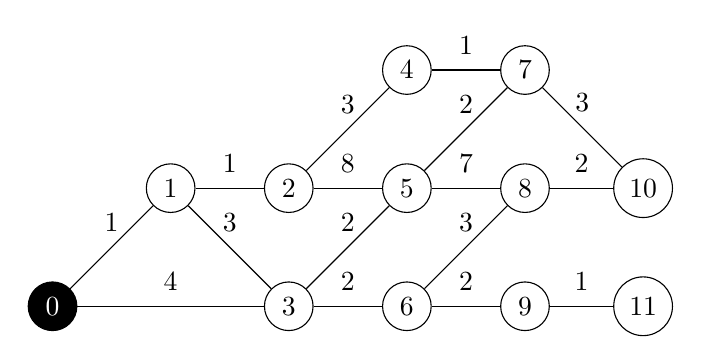
\begin{tikzpicture}
\node[circle,draw,fill=black,text=white] (s) at (0,0)  {0};
%\node[left=1em] {$s$};
\node[circle,draw] (a) at (1.5,1.5) {1};
\node[circle,draw] (b) at (3,1.5)   {2};
\node[circle,draw] (c) at (3,0)   {3};
\node[circle,draw] (d) at (4.5,3)   {4};
\node[circle,draw] (e) at (4.5,1.5)   {5};
\node[circle,draw] (f) at (4.5,0)   {6};
\node[circle,draw,fill=white] (g) at (6,3)   {7};
\node[circle,draw,fill=white] (h) at (6,1.5)   {8};
\node[circle,draw,fill=white] (i) at (6,0)   {9};
\node[circle,draw,fill=white] (j) at (7.5,1.5)   {10};
\node[circle,draw,fill=white] (k) at (7.5,0)   {11};
\draw (s) edge node[above=2pt] {1} (a);
\draw (s) edge node[above=2pt] {4} (c);
\draw (a) edge node[above=2pt] {1} (b);
\draw (a) edge[-] node[above=2pt] {3} (c);
\draw (b) edge node[above=2pt] {3} (d);
\draw (c) edge node[above=2pt] {2} (e);
\draw (c) edge node[above=2pt] {2} (f);
\draw (b) edge[-] node[above=2pt] {8} (e);
\draw (d) edge[-] node[above=2pt] {1} (g);
\draw (e) edge[-] node[above=2pt] {2} (g);
\draw (e) edge[-] node[above=2pt] {7} (h);
\draw (f) edge[-] node[above=2pt] {3} (h);
\draw (f) edge[-] node[above=2pt] {2} (i);
\draw (g) edge[-] node[above=2pt] {3} (j);
\draw (h) edge[-] node[above=2pt] {2} (j);
\draw (i) edge[-] node[above=2pt] {1} (k);
\end{tikzpicture}
\end{document}